%% uctest.tex 11/3/94
%% Copyright (C) 1988-2004 Daniel Gildea, BBF, Ethan Munson.
%
% This work may be distributed and/or modified under the
% conditions of the LaTeX Project Public License, either version 1.3
% of this license or (at your option) any later version.
% The latest version of this license is in
%   http://www.latex-project.org/lppl.txt
% and version 1.3 or later is part of all distributions of LaTeX
% version 2003/12/01 or later.
%
% This work has the LPPL maintenance status "maintained".
% 
% The Current Maintainer of this work is Daniel Gildea.
%
% 2007/08/01
% LaTeX Package "ucr" is modified from LaTeX package "ucthesis."
% This modification is therefore under to the conditions of 
% the LaTeX Project Public License.
% Its formality is suitable for the dissertation of Universty of
% California, Riverside.
% This test document is for the convenience of all students of
% Universty of California, Riverside.
% Contact Charles Yang at chcyang@yahoo.com if you like.
% Charles Yang has nothing to do with the original author's sarcasm.
%
% \documentclass[11pt]{ucthesis}
% \documentclass[11pt]{ucr}
\documentclass[oneside,final, letterpaper]{ucr}
\begin{document}

% Declarations for Front Matter

\title{Neural Network-based Embedding generation using Program Dependency Graph for Binary Code Similarity Detection.}
\author{Abhishek Kumar Srivastava}
\degreemonth{June}
\degreeyear{2018}
\degree{Master of Science}
\chair{Dr. Heng Yin}
\othermembers{Dr. Vagelis (Evangelos) Papalexakis\\
Dr. Silas Richelson}
\numberofmembers{3}
\field{Computer Science}
\campus{Riverside}

\maketitle
\copyrightpage{}
\approvalpage{}

\degreesemester{Fall}

\begin{frontmatter}

\begin{acknowledgements}
. . .
\end{acknowledgements}

\begin{dedication}
\null\vfil
{\large
\begin{center}
. . . %To my parents and friends for all the support and keeping me sane during though times.
\end{center}}
\vfil\null
\end{dedication}

\begin{abstract}

Analyzing software binaries can be helpful in tackling important problems such as plagiarism, malware or vulnerability detection. Detecting similarity between two binary functions coming from different sources can be done using binary code similarity detection. Existing approaches use Control-Flow graph information of binaries in some way or another \textit{i.e} either graph matching or control-block embedding which is either slow or does not utilize all the information. In this work we propose novel way to use program dependency graph of functions to extract control and data dependency information and generate its embedding with help of Neural Network using this information. Measuring the distance between embedding of different binary functions can evaluate their similarity. Since this method does not rely on internal flow structure of the function it can be applied to more generally and is resilient to different compiler optimizations and heavy obfuscation techniques.
\end{abstract}

\tableofcontents
\listoffigures
\listoftables
\end{frontmatter}

% \part{First Part}


\chapter{Introduction}
Today software applications in some form or another is used in every aspect of our lives. Softwares are being constantly developed to handle more complex issues while being scalable to millions of users and due to this complexity involved in development they may suffer from serious software implications such as exploitable malwares \& vulnerabilities. The study by Cui et al. showed that 80.4\% of vendor-issued firmware is released with multiple known vulnerabilities, and many recently released firmware updates contain vulnerabilities in third-party libraries that have been known for over eight years \cite{Cui}. 

Most malware's developed today are not created from scratch but in some way they are modification of some existing malware to create new ones. This can be used to our advantage by using code reuse detection to generate feature vectors for those and use with machine learning algorithms that can recognize new or similar malware or vulnerabilities \cite{Jang}. One of the other reason for analyzing binaries for finding vulnerabilities and plagiarism are often lack of source code because of third-party software \cite{Saeb} or not having access of source codes we wish to perform analysis on but almost everyone having access to binary (i.e., executable) code. Binary analysis is thus important for understanding the inner workings of malware or exploring vulnerabilities in existing systems but doing it manually is a very intensive task. Due of these challenges binary analysis is an very important area of research in computer science and automated tools which can do the analysis efficiently and effectively are in very high demand.

\section{Background}

Recently, there has been bloom in research to tackle the problem of binary code similarity detection. In binary code analysis detecting similar functions in binary executables remains one of the fundamental problem and is well known as ``binary code similarity detection'' problem. These efforts commonly involves extracting binary code into representable form either a vector or graph to represent functions of binary.  Then, it is checked that whether among extracted control flow graph functions representations any functions are similar or not using a graph matching algorithm.  

%since we are generally missing abstractions provided by programming languages making 
%binary analysis difficult \cite{Teresa} but there are some advantages 

Graph-based matching approaches have some drawbacks. One of them is their adaptability for different applications since they are approximated by fixed graph matching algorithm. For example, even the same code compiled with different optimization level may result in producing different control flow graphs since it will be not be matched by fixed graph matching\cite{Xu}. Other problem is due to inefficiency of graph matching algorithm (such as bipartite graph mathcing) which are considerably slow thus it will degrade the overall efficiency of code similarity detection since it heavily rely on the graph matching algorithm.  

A practical and efficient clone searching algorithm relies on a robust vector representation of assembly code. However, existing clone search approaches, rely on a manual feature engineering for every assembly function process to create its vector representation,which fail to identify unique patterns that can statistically distinguish assembly functions. However, it is a challenging problem to automatically pick the best representation of a function due to the fact that there are varieties of compiler optimizations and code obfuscation techniques that make equivalent assembly functions appear to be very different. These techniques have a strong impact on the resulting assembly instructions and the linear layout of the assembly code. Figure 1.1 shows some examples of assembly functions that correspond to the same source code. The major challenge is how to identify these semantically equivalent but structurally different assembly functions as clones.


\begin{figure}
	\centering
	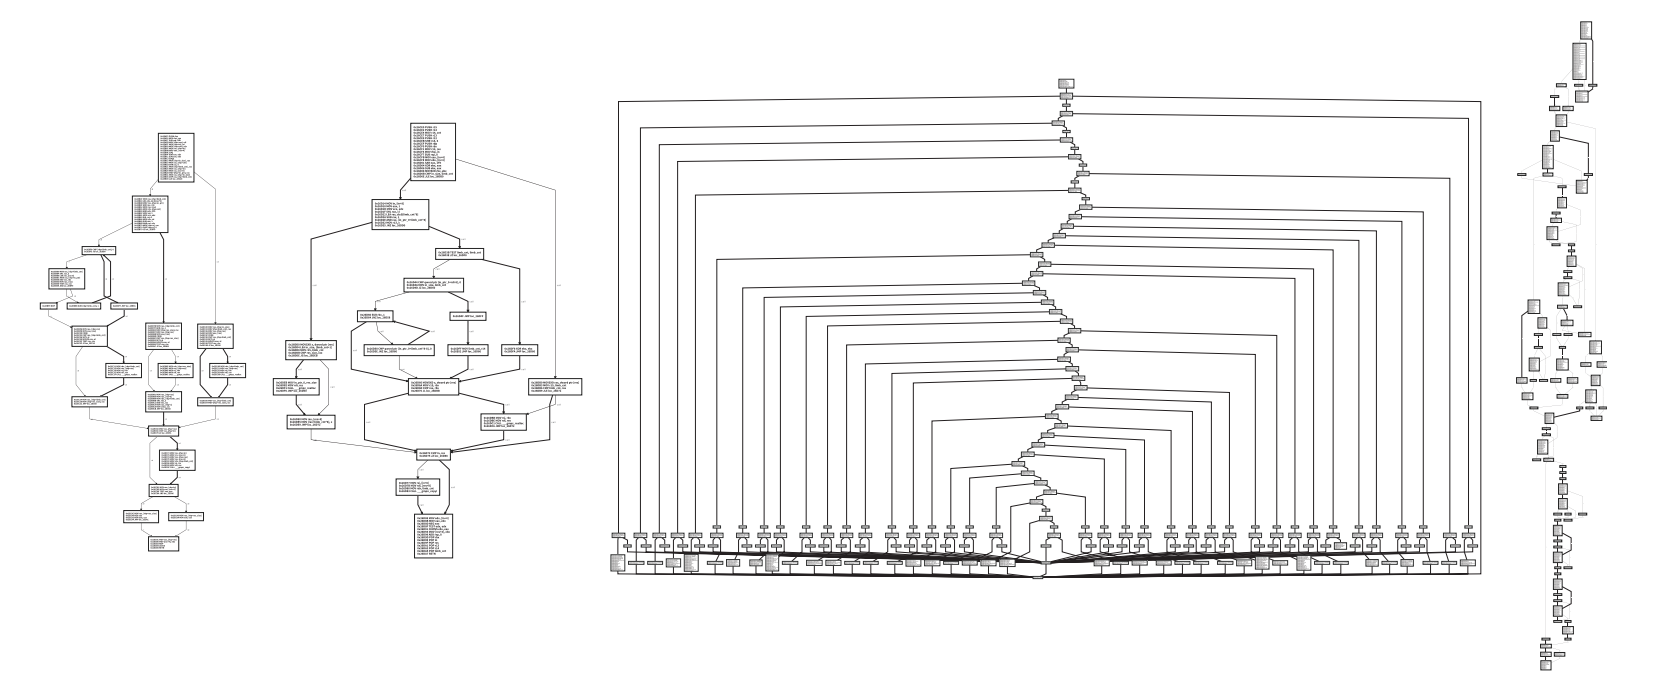
\epsfig{file=diff_cfgs.png, height=2.75in, width=6.5in}
	\caption{Different assembly functions compiled from the same \textit{gmpz\_tdiv\_r\_2exp} function of \textit{Libgmp}. From left to right, the assembly functions are compiled with the \textit{GCC O0} option, \textit{GCC O3} option, \textit{Obfuscator-LLVM} Control Flow Graph Flattening option and Bogus Control Flow Graph option.}
\end{figure}


Typically, the following four categories of features are used in the literature for assembly clone search.

\textbf{Token-based features :} These features model the similarity between two assembly code functions based on a set of tokens. The tokens can include constants, assembly instructions such as n-grams or n-perms \cite{Khoo}, or assembly instructions with normalized operands
\cite{Ding, Farhadi, Andreas}. Typically, the frequency value is used to construct the feature vector. Constant tokens are robust if they are weighted correctly. Some common constants such as the ones used for stack manipulation are insufficient to distinguish assembly functions, which leads to a relatively lower level of recall rate as shown in \cite{Khoo}. Instruction-based tokens have a weak robustness since the selected compiler, compiler optimization settings, and the obfuscation techniques all have a strong influence on the choice of instructions. The same logic can be expressed differently in assembly code. More importantly, instruction tokens used as features fail to capture the semantic relationship between tokens. For example, the assembly instructions Add and Sub are similar in the sense that they are both arithmetic instructions. To address this problem, in [7, 9] instructions are classified into categories such as transfer, algorithmic, and stack operations, among others. However, they fail to model the relationship between instructions across different categories. The best way is to learn the relationship directly from data. Let the assembly code itself show what assembly instructions are similar by considering the context in which they co-occur. For example, instructions appearing around stack registers are similar as they somehow relate to stack manipulation. Likewise, instructions appearing around floating point registers are similar in the sense that they somehow relate to floating point operations and vice versa.

\textbf{Text-based features :} Studies such as \cite{David} fall into this category. It models the similarity between two assembly functions or frag- ments based on a customized string editing distance. String editing distance is not robust, since the linear layout of the assembly code
can be modified  easily. Obfuscator can substitute instructions with their semantically equivalent but syntactically different form, which leads to a very different editing distance. A good representation of assembly code should be able to identify position-invariant patterns
that is robust to different linear layouts.

\textbf{Graph-based features :} Studies under this category compare assembly functions using subgraph isomorphism algorithms \cite{Ding, Eschweiler, Pewny} or a set of graph substructures \cite{Feng, Khoo, Kruegel} as features. Graph-based features rely on the correct detection of basic block boundaries
and reconstruction of Control Flow Graphs (CFG). Graph-based features are not robust, since different compiler optimization settings can already significantly change the control flow graph by loop unrolling and function inlining. Some approaches use subgraphs that consists of 2-3 nodes as features \cite{Khoo, Kruegel}. Their robustness is therefore enhanced. Even if the CFG is heavily modified, some important logics and subgraph structures still remain the same.
These features are less sensitive to CFG modifications. However, a graph flattening obfuscation technique from Obfuscator-LLVM (O-LLVM) \cite{Junod} that destroys all the subgraph structures can make
the graph-based features useless.

\textbf{Dynamic features :} Studies under this category dynamically execute fragments of assembly code and use them as features \cite{Chandramohan, David, Pewny}. These features normalize assembly instructions that are semantically equivalent but syntactically different. However, one of the main problems is that it requires a pair-wise full permutation of  input/output variables to match the symbolic expressions extracted from the assembly code. This process is slow and can hardly be scalable without developing a specialized indexing schema for symbolic expression. Moreover, different assembly instructions have different side effects such as setting the flag bits. When matching assembly functions, it is difficult to determine what is the main logic and what would be the correct set of input and output. 


All the aforementioned approaches are based on the manual feature engineering process, several assumptions are made. Thus, the chosen representation may not truly embrace the important patterns that distinguish one assembly function from another. Deep learning \cite{LeCun} in recent years has be involved in many application domains which also includes binary analysis and has concluded pretty interesting results than other approaches. Deep learning allow us to learn representations of data(vector or graphical) with multiple levels of abstraction freeing involvement of any domain knowledge which is very big advantage of using it. It is also very adaptive and can be modified to train on data of our particular interest and can be utilized in our approach.

\section{Purpose}

We propose a novel approach, for assembly clone detection. It is different from graph-based methods since we first extracts the information from the binaries and feed this information to Neural Network to generate an embedding (vector representation) of the functions. All previous research on assembly code clone relies on the manual feature engineering process. Our vector representation of assembly code as a way to mitigate the afore mentioned issues in current handcrafted features. Combining the graph embedding networks into a Siamese network \cite{Bromley} naturally captures the objective that the graph embeddings of two similar functions should be close to each other and vice versa. This entire network model can then be trained end-to-end for similarity detection. Further, we design a new training and dataset creation method using a default policy to pre-train a task-independent graph embedding network. The learning process does not also require any prior knowledge about assembly code, such as compiler optimization settings or the correct mapping between assembly functions. It only needs assembly code functions. We discuss the differences between the assembly code and text data, as well as the issues we had in applying the representation learning on assembly code.

Our approach constructs a large-scale training dataset using binary functions compiled from the same source code but for different platforms and compiler optimization levels. Our evaluation demonstrates that this task-independent model is more effective and generalize better to unseen functions than the state-of-the-art graph matching-based approach \cite{Dullien}. One advantage of the neural network-based approach is that the pre-trained model can be retrained quickly in the presence of additional supervision to adapt to new application scenarios. Our evaluation shows that with such additional supervision, the retrained model can efficiently adapt to novel tasks. This efficiency property enables practical usage of the retraining to improve the quality of similarity detection. We have implemented a prototype called Gemini. In a broader scope, this work showcases a successful example of how to apply deep learning to solve important and emerging computer security problems and substantially improves over the
state-of-the-art results. We conduct extensive experiments with all the combinations of optimization levels in the GNU GCC compiler. We benchmark various state-of-the-art assembly clone search techniques in the experiment. We show that by using representation learning, a simple cosine-similarity-based approach significantly outperforms the others regarding both recall and precision.

%and different obfuscation techniques of Obfuscator-LLVM [14] with the CLANG compiler. It is the first clone search experiment that covers a strong obfuscator which substitutes instructions, splits basic blocks, adds bogus logics, and completely destroys the original control flow graph.
 

\section{Outline}
We summarize our contributions as follows:

\begin{itemize}
	\item We propose the neural network-based approach to generating embeddings for binary functions.
	\item We propose a novel approach to train the embedding network using a Siamese network so that a pre-trained model can generate embedding to be used for similarity detection.
	\item We propose a retraining approach so that the pre-trained 	model can take additional supervision to adapt to specific tasks.
	\item We implement a prototype and our evaluation demonstrates that on a test set constructed from OpenSSL, it can achieve a higher AUC than previous state-of-the-art graph matching-based approach;
\end{itemize}


The rest of the thesis is organized as follows. Chapter 2 gives detailed introductions to several different topics that is used throughout the thesis. Chapter 3 contains describes the approach and an overview of implementation used for the binaries analysis required by this project. Chapter 4 presents results obtained during the evaluation of the system developed Finally, Chapter 5 presents conclusions regarding binary analysis based code similarity detection of with suggestions for future work.
 %usually intro
\chapter{Theory}
\section{Binary Disassembly}

An assembly language is a programming language that is very close to the actual machine code that is interpreted by a processor. Instead of ones and zeroes however, an assembly language uses mnemonics, or abbreviations, for the instructions available for the computer architecture. An important aspect of the assembly language in the context of disassembly is that there is a one-to-one mapping between assembly language instructions and instructions in machine code. This means there can be no  ambiguities when translating instructions from the assembly language to machine code or from machine code back to the assembly language, although the latter requires an understanding of the control flow structure of the binary program.

There are a few different dialects of the x86 assembly language, and most notable is the Intel syntax and the AT\&T syntax. The most important differences between these two dialects is (a) the parameter order where Intel places destination before source and AT\&T places source before the destination, (b) that mnemonics in the AT\&T syntax are suffixed with a letter to indicate the size of the operation whereas this information is derived from the register that is used in the Intel syntax and (c) the general syntax for effective addresses.

Disassembly is the process of transforming a set of machine code instructions, a binary file, into a set of assembly instructions. It is the exact opposite of the assembler process which is usually the last step when compiling a program from source code \cite{Aho, Linn}. Disassembly can either be performed as a static process, where the set of machine code instructions that are being disassembled are never executed, or as a dynamic process, where the set of assembly instructions that constitutes the machine code is extracted during execution \cite{Linn}. Static disassembly has the advantage of processing an entire set of machine code instructions at once while dynamic disassembly can only process the subset of machine code instructions that are actually executed. Dynamic disassembly on the other hand has the advantage of extracting a sequence of instructions that is guaranteed to be correct for the execution during which it was extracted.

Decompilation, is the process of transforming a set of machine code instructions, or a set of assembly instructions, into a representation in a high-level language \cite{Cifuentes}. The purpose is to reconstruct the source code of the binary program in a high-level language that can easily be read and understood by a human in order to audit the code or make changes to the functions of the program. Decompilation is a process that is usually performed after disassembly and applies additional transformations to the assembly instructions produced by the disassembly process, thus it should not be seen as a conflicting process to disassembly.

In order to decompile a program correctly, the program’s control flow paths needs to be known, or discovered, during the process. Dynamically, this information can be obtained for the subset of instructions that is actually executed while the program is being monitored. Statically the entire program will be processed, but there will be ambiguities in the result since not all information regarding the control flow can be known in a static context.

The reason for these ambiguities that arises when statically reconstructing the control flow of a binary files stems from the fact that there is more information present in the original source code. This additional information which primarily concerns control flow is removed when the program is compiled into an executable binary since the information is not needed in order for the program to execute correctly. Fully structured code, where every control-structure has a single point of entry and a single point of exit, should have considerably less ambiguities. This is because once a point of entry is found, the point of exit can be known immediately.

The modern computer programs are developed in programming languages that are a human readable form \cite{Agrawal, Kargen, Allen}. The source code written by software developers is compiled into a binary format. In software development, there are two classes of binaries: 

\begin{itemize}
	\item \textbf{Machine code }- is not directly understandable by software developer, but it is directly executed by the machine; it is generated by compiler depending on the hardware characteristics;  
	\item \textbf{Intermediate code }- like machine code, is not directly understandable by software developer and is not directly executed by the machine; the executable code is obtained  after an interpreting process performed by a specialized component called virtual machine; the most known and used virtual machines are Java Virtual Machine and Common Language Runtime (CLR) \cite{Fer, Cytron}.
\end{itemize}


The computer programs delivered in the machine code format are more difficult to be maintained because of the difficulty to understand the executable format. To implement the maintainance activities, the software developer need the source code and documentation. Another way to obtain the understandable form of the machine code is to convert it into assembly language.

The practical and positive issues of the disassembly process and its results are :

\begin{itemize}
	\item Improvement of the portability for computer programs delivered in machine code format; unlike machine code, the intermediate code is portable due to its interpreting by a virtual machine which must be mandatorily installed on the host machine;
	\item The software developers determine the logical flows of the disassembled software application; the algorithms and other programming entities are extracted from the software application and used in other versions or programs;
	\item Security issues are identified and can be patched without access to the original source code;
\end{itemize}

As negative issue, the disassembly process can be carried out by malicious software developers to discover the vulnerabilities and holes of the computer programs to hack them. Also, the discovered logical flows and algorithms can be used in other commercial computer programs without an agreement with the owners of the disassembled computer program.

The list of the available disassemblers includes tools for Windows like IDA Pro, PE Explorer, W32DASM, BORG Disassembler, HT Editor, diStorm64 and Linux like Bastard Disassembler, ciasdis, objdump, gdb, lida linux interactive disassembler, ldasm.

\section{Control Flow Graphs}

A control flow graph (CFG) is a directed, connected, graph that is used to represent all possible paths of execution that can occur within a program. Each vertex in the control flow graph represents a basic block, a linear sequence of instructions, and each edge between two vertices represents a possible control flow path \cite{Allen}. A control flow graph has two artificial vertices, $v_{START}$ and $v_{END}$ . The reason for these two artificial vertices is to ensure a connected graph where every actual vertex without a predecessor is is connected with $v_{START}$ and every actual vertex without a successor is connected with $v_{START}$ . Because of this addition to the graph there is a path $v_{START}$ ...$v$...$v_{END}$ for every vertex $v$ within the graph.

For the purpose of explaining a control flow graph, instructions can be classified either as a Transfer Instruction (TI) or as a Non Transfer Instruction (NTI). Transfer instructions are the set of instructions that might transfer control flow to a part of the program different from the address of the next instruction. Unconditional jumps, where the control flow is transferred to the
target jump address; conditional jumps, where the control flow might be transferred to the target jump address; and subroutine calls, where the control flow is transferred to the invoked subroutine, are all examples of transfer instructions. Non transfer instructions are the set of instructions that will always transfer the control flow to the next instruction in sequence [6].

A basic block is a sequence of instructions that has a single point of entry and a single point of exit. A basic block either consists of zero or more non transfer instructions and ends with a single transfer instruction or consists of one or more non transfer instructions.

In addition to the classifications made by Cristina Cifuentes in [6], call basic block that has an indirect address reference (calculated during runtime), will be treated as if they had no outgoing edges. The reason for this addition to the classifications is to preserve context sensitivity when performing dynamic analysis. Context sensitivity in binary analysis is the concept that a function’s
behavior, and impact on the program, is relative to the calling context, or in other words, relative to the part of the code that called the function. Since functions are only control-dependent on a specific call-instruction as long as that instruction is part of the code that is currently being executed, adding edges to a function from each call would result in erroneous control-dependencies.

\section{Program Dependency Graphs}

The PDG makes explicit both the data and control dependences for each operation in a program. Data dependence graphs have provided some optimizing compilers with an explicit representation of the definition-use relationships implicitly present in a source program. A control flow graph has been the usual representation for the control flow relationships of a program; the control conditions on which an operation depends can be derived from such a graph.

Since both kinds of dependences are present in a single form, transformations like vectorization can treat control and data dependence uniformly. Program transformations such as code motion, which require interaction of the two types of dependences, can also be easily handled by our single graph.


\subsection{Control Dependency Graphs}
A control dependence graph (CDG) is a partially ordered, directed, acyclic graph where the vertices of the graph represents basic blocks and the edges between two vertices represents the control conditions on which the execution of the operations depends [10]. A control dependence between two vertices in a control flow graph exists if there is a conditional branch at one of the vertices
(the source of the dependence) that determines whether or not the other vertex (the sink of the dependence) is to be executed.

A vertex v q is control dependent on a vertex v p if (a) v q 6 = v p , (b) v q does not post-dominate v p and (c), there exists a path from v p to v q such that v q post-dominates every vertex on the path except for v p . A vertex v q can be control dependent on itself if there exists a path from v q to v q such that v q post-dominates every vertex on the path.

A static control dependence graph can contain fewer vertices than the initial control flow graph since there is no need to keep vertices in the static control dependence graph if they (a) depend on the same vertex as their immediate dominator and (b) doesn’t have any vertices depending on them. That being said, a static control dependence graph can still be larger than the initial control flow graph in terms of edges since a single vertex can be control dependent on hundreds or even thousands of vertices.

A dynamic control dependence graph, like its static counterpart, can contain fewer vertices than the initial control flow graph. Although, every vertex that controls whether or not another executed vertex should be executed, and every executed vertex that is control dependent on another vertex will be part of the dynamic control dependence graph. The maximum number of edges in a
dynamic control dependence graph is unbounded since almost every transition of control flow from one vertex to another will yield a new edge from the executed vertex to the vertex that it is control dependent upon.


\subsection{Data Dependency Graphs}
In this section we describe how DDGs are represented, starting with the logical graph representation. We then briefly outline our physical representation, and discuss how
graphs are traversed.

Data dependence analysis determines what the constraints are on how a piece of code can be reorganized.

Data dependences are constraints on the order in which statements may be execute.

Data dependencies may be represented using a directed acyclic graph (DAG).

Nodes are machine instructions. Edge i -> j if instruction j has a data dependence on instruction i.

Logical graph representation. Let I and J be two instructions in a program, and i, j be execution instances of I and J, respectively. i has a data dependency on j if i
uses data defined by j.

In the classical graph representation used in early works, such as, instruction instances are represented by vertices, and data or control dependencies are represented by outgoing
edges from vertices. We instead use a graph representation similar to the one proposed by Zhang
and Gupta in [8]. In their graphs, each static instruction is represented by a vertex, and data or control dependencies are represented by adding labeled edges between vertices.
The number of vertices is thus bounded by the size of the program, while the number of edges per vertex is determined by the length of execution. The label of an edge identifies the instruction instances involved in the corresponding dependency. For example, a data dependency of i on j is represented by adding an edge from I to J, labeled with instance(i) and instance(j)
i.e. the use-instance of I and the define-instance of J.


\section{Neural Network}
Neural networks are a set of algorithms, modeled loosely after the human brain, that are designed to recognize patterns. They interpret sensory data through a kind of machine perception, labeling or clustering raw input. The patterns they recognize are numerical, contained in vectors, into which all real-world data, be it images, sound, text or time series, must be translated.

Neural networks help us cluster and classify. You can think of them as a clustering and classification layer on top of the data you store and manage. They help to group unlabeled data according to similarities among the example inputs, and they classify data when they have a labeled dataset to train on.

Neural neworks are typically organized in layers. Layers are made up of a number of interconnected 'nodes' which contain an 'activation function'. Patterns are presented to the network via the 'input layer', which communicates to one or more 'hidden layers' where the actual processing is done via a system of weighted 'connections'. The hidden layers then link to an 'output layer' where the answer is output. Most ANNs contain some form of 'learning rule' which modifies the weights of the connections according to the input patterns that it is presented with. In a sense, ANNs learn by example as do their biological counterparts

he delta rule is often utilized by the most common class of ANNs called 'backpropagational neural networks' (BPNNs). Backpropagation is an abbreviation for the backwards propagation of error.

With the delta rule, as with other types of backpropagation, 'learning' is a supervised process that occurs with each cycle or 'epoch' (i.e. each time the network is presented with a new input pattern) through a forward activation flow of outputs, and the backwards error propagation of weight adjustments. More simply, when a neural network is initially presented with a pattern it makes a random 'guess' as to what it might be. It then sees how far its answer was from the actual one and makes an appropriate adjustment to its connection weights. Backpropagation performs a gradient descent within the solution's vector space towards a 'global minimum' along the steepest vector of the error surface. The global minimum is that theoretical solution with the lowest possible error. The error surface itself is a hyperparaboloid but is seldom 'smooth'.  Indeed, in most problems, the solution space is quite irregular with numerous 'pits' and 'hills' which may cause the network to settle down in a 'local minum' which is not the best overall solution. Since the nature of the error space can not be known a prioi, neural network analysis often requires a large number of individual runs to determine the best solution. Most learning rules have built-in mathematical terms to assist in this process which control the 'speed' (Beta-coefficient) and the 'momentum' of the learning. The speed of learning is actually the rate of convergence between the current solution and the global minimum. Momentum helps the network to overcome obstacles (local minima) in the error surface and settle down at or near the global miniumum.

Once a neural network is 'trained' to a satisfactory level it may be used as an analytical tool on other data. To do this, the user no longer specifies any training runs and instead allows the network to work in forward propagation mode only. New inputs are presented to the input pattern where they filter into and are processed by the middle layers as though training were taking place, however, at this point the output is retained and no backpropagation occurs. The output of a forward propagation run is the predicted model for the data which can then be used for further analysis and interpretation.

It is also possible to over-train a neural network, which means that the network has been trained exactly to respond to only one type of input; which is much like rote memorization. If this should happen then learning can no longer occur and the network is refered to as having been "grandmothered" in neural network jargon. In real-world applications this situation is not very useful since one would need a separate grandmothered network for each new kind of input.

However they work very well for:
capturing associations or discovering regularities within a set of patterns;
where the volume, number of variables or diversity of the data is very great;
the relationships between variables are vaguely understood; or,
the relationships are difficult to describe adequately with conventional approaches.


There are many advantages and limitations to neural network analysis and to discuss this subject properly we would have to look at each individual type of network, which isn't necessary for this general discussion.

Backpropagational neural networks (and many other types of networks) are in a sense the ultimate 'black boxes'. Apart from defining the general archetecture of a network and perhaps initially seeding it with a random numbers, the user has no other role than to feed it input and watch it train and await the output. In fact, it has been said that with backpropagation, "you almost don't know what you're doing". Some software freely available software packages (NevProp, bp, Mactivation) do allow the user to sample the networks 'progress' at regular time intervals, but the learning itself progresses on its own. The final product of this activity is a trained network that provides no equations or coefficients defining a relationship (as in regression) beyond it's own internal mathematics. The network 'IS' the final equation of the relationship.

Backpropagational networks also tend to be slower to train than other types of networks and sometimes require thousands of epochs. If run on a truly parallel computer system this issue is not really a problem, but if the BPNN is being simulated on a standard serial machine (i.e. a single SPARC, Mac or PC) training can take some time. This is because the machines CPU must compute the function of each node and connection separately, which can be problematic in very large networks with a large amount of data. However, the speed of most current machines is such that this is typically not much of an issue.

\subsection{Siamese Architecture}
Siamese networks are a special type of neural network architecture. Instead of a model learning to classify its inputs, the neural networks learns to differentiate between two inputs. 

A Siamese networks consists of two identical neural networks, each taking one of the two input images. The last layers of the two networks are then fed to a contrastive loss function , which calculates the similarity between the two images. There are two sister networks, which are identical neural networks, with the exact same weights. Each image in the image pair is fed to one of these networks. The networks are optimised using a contrastive loss function. The objective of the siamese architecture is not to classify input images, but to differentiate between them. So, a classification loss function (such as cross entropy) would not be the best fit. Instead, this architecture is better suited to use a contrastive function. Intuitively, this function just evaluates how well the network is distinguishing a given pair of images.

Similarity learning with deep CNNs is typically addressed using Siamese architectures.

For this domain, we
employ large siamese convolutional neural networks which a) are capable of learning generic image features useful for making predictions about unknown class distributions
even when very few examples from these new distributions are available; b) are easily trained using standard optimization techniques on pairs sampled from the source
data; and c) provide a competitive approach that does not rely upon domain-specific knowledge by instead exploiting deep learning techniques.

Siamese nets were first introduced in the early 1990s by Bromley and LeCun to solve signature verification as an image matching problem. A siamese neural network consists of twin networks which accept distinct inputs but are joined by an energy function at the top. This function computes some metric between the highestlevel feature representation on each side. The
parameters between the twin networks are tied. Weight tying guarantees that two extremely similar images could not possibly be mapped by their respective networks to very different locations in feature space because each network computes the same function. Also, the network is symmetric, so that whenever we present two distinct images to the twin networks, the top conjoining layer will compute the same metric as if we were to we present the same two images
but to the opposite twins.

\chapter{Approach}
\section{Raw Feature Extraction}
\subsection{CFG Features}
\subsection{PDG Features}
\section{Neural Network Model}
\subsection{Hyperparameters}
\chapter{Evaluation}
\section{Implementation and Setup}
\subsection{Sample Generation}
\subsection{Training Details}
\section{Accuracy}
\subsection{CFG-Based}
\subsection{PDG-Based}
\section{Efficiency}
\subsection{CFG-Based}
\subsection{PDG-Based}

\chapter{Conclusions}




%\nocite{*}
% \singlespacing
\bibliographystyle{plain}
\bibliography{bibfile}

\appendix



\end{document}
